\documentclass{article}
\usepackage[a4paper,top=3.5cm,bottom=5cm,left=3.8cm,right=3.8cm,marginparwidth=1.75cm]{geometry}
\usepackage{graphicx} % Required for inserting images
\usepackage{float}
\usepackage{hyperref}
\usepackage{subcaption}

\usepackage{cite}

\title{\textbf{Generating Street View Images with a GAN}\\Assignment 2 - Final Project\\Advanced Deep Learning Modes}
\author{Eric Roy}
\date{March 2025}

\begin{document}

\maketitle

\section{Introduction}

This report presents a Deep Convolutional Generative Adversarial Network (DC-GAN) trained to be
able to generate images that look like Google Street View data.
This is the final project of the Advanced Deep Learning Modes course, and had an 8-hour
time limit.

\section{Dataset used}

To train a model like the previously mentioned we need a dataset. The one that got chosen was 
\cite{google_street_view_dataset}. This dataset
contains 10k images of Google Street View, and the exact coordinates where they've been taken.
The dataset is organized with a directory with all of the images and a CSV file with the 
coordinates and the file name, to be able to retrieve the location of the pictures.

Since all of these images have been taken by Google with the (almost) same equipment, the
dataset is consistent. All images have the same size ($640\cdot640$ px), and the coordinates reflect the exact
location with no (or only little) errors. An example of the input images can be seen in
Figure \ref{fig:input}.

\subsection{Coordinate distribution}

This would allow to filter images by, for example, country. However, by doing that I found out
that there were almost no images in North-America, which is weird due to the fact that Google is
based in the USA. To get a general view of where the images of the dataset are I decided to plot them in a world map using the Python library \textit{cartopy}. The world map can be seen in Figure 
\ref{fig:worldmap}.

Figure \ref{fig:worldmap} shows clearly some properties of bad datasets. The main one is that the images are not uniformly distributed across all over the world. This is a bad thing because now it's even more difficult because the GAN will not be able to generate images from the missing countries, and it will be hard to create models for a specific region.

\subsection{Dataset expansion}

After the previously seen results it would be a good solution to find another dataset, or to
create one on our own. However, given the time limit of this project, this won't be possible.

It is still interesting to point the reader to the Google Street View API \cite{streetViewAPI}
to get first-hand images from less randomized regions.

\subsection{Data augmentation}

To prevent overfitting and get more training data I used data augmentation to randomly zoom into
some images and crop them, all while maintaining the original width and height.

\section{Training}

To train easily the generator and discriminator I created a script that can be customized from
the command line arguments. For example, training can be resumed from a certain epoch, and models
are saved every 10 epochs. The image region can also be selected, with some as examples, but
the previous data distribution problem has made this setting useless (with the current dataset).

The model architecture doesn't have any secret. There are a lot of \texttt{Conv2DTranspose} layers
to make the generator go from a $l=100$ random noise array to the $640$ pixel image, and some
Convolutions with a dense layer at the end to make the discriminator. The loss function is
binary Cross-Entropy, and I've used Adam as an optimizer.

Some quick tests demonstrated that the model needed a lot of epochs to generate some
useful output, and it was trained on the UPC's server for 250 epochs (3 minutes per epoch, using
only one GPU). I used Mini-Batch Gradient Descend, but I had to reduce the batch size from 64 to
32 due to the fact that i ran out of GPU memory.

Looking back at this procedure I should've tried smaller images with a bigger batch size to first
see if the model could converge correctly, before training the model with big images at first.

\section{Results}

The results of this training process were rather disappointing. We can see in Figure \ref{fig:results} the results after some epochs. Although the model can successfully generate
the skyline and some trees, the resolution is very bad.
To train the last 50 epochs I did reset the discriminator model, which seems to have had a good impact, given the change between the last two images of Figure \ref{fig:results}.

\section{Conclusions and future work}

Although the results might not be the best, I still have managed to create a GAN on Google Street View images that, in some specific epochs, did create some interesting images. However, the poor dataset quality and some bad decisions during the architecture design led to improvable results.

Future work on this project might involve training again the model but with lower-resolution images. This way there are less parameters, and the batch size can be increased. The dataset can also be improved to prevent overfitting and be able to train the model with only specific regions of the world. Finally, the last improvement would be to tweak the learning rate and other hyperparameter of the DC-GAN.

As an end note, it's worth mentioning two projects on a similar field that could be interesting to combine with this one. These are \cite{streetViewAI1} and \cite{streetViewAI2}. Both of them are Convolutional Neural Networks (CNN) that predict the location of a Google Street View Image. It would be fun to try to predict the location of one of the generated images.

\bibliography{mybib}{}
\bibliographystyle{apalike}

\begin{figure}[H]
    \centering
    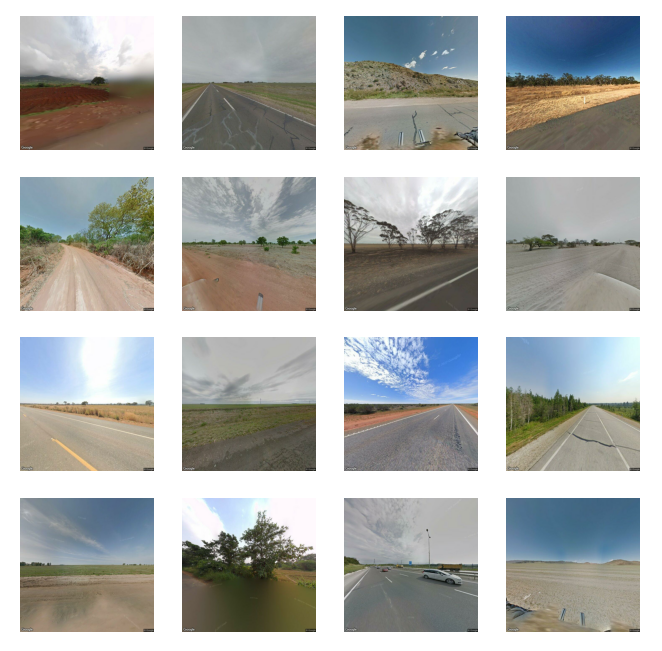
\includegraphics[width=0.7\linewidth]{input.png}
    \caption{Sample of the images in the dataset}
    \label{fig:input}
\end{figure}

\begin{figure}[H]
    \centering
    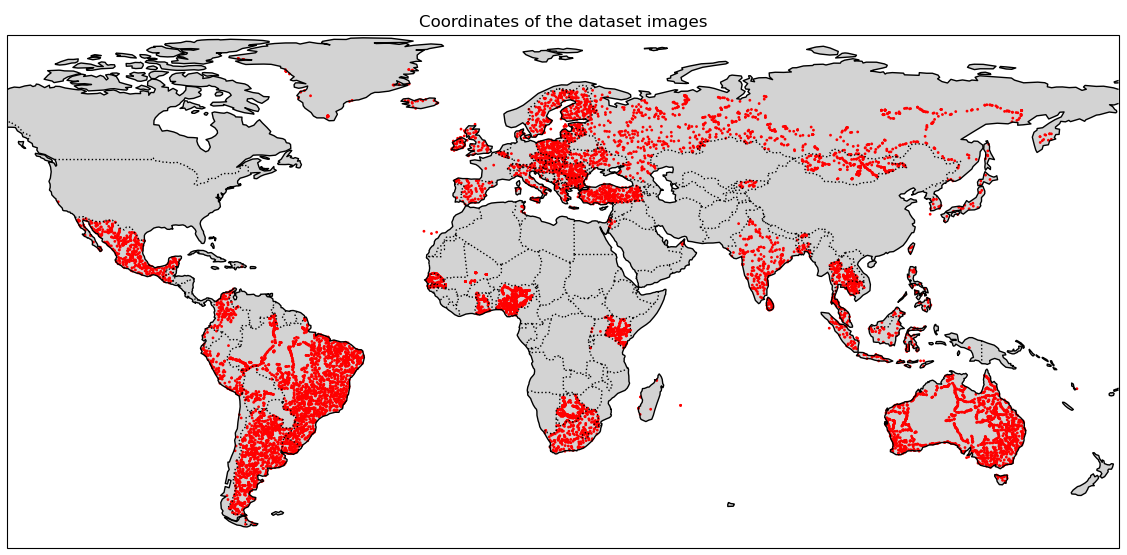
\includegraphics[width=0.9\linewidth]{coordinates.png}
    \caption{Coordinates of each Street View image on the dataset.}
    \label{fig:worldmap}
\end{figure}

\begin{figure}[H]
    \centering
    \begin{tabular}{cccc}
        \begin{subfigure}{0.23\textwidth}
            \centering
            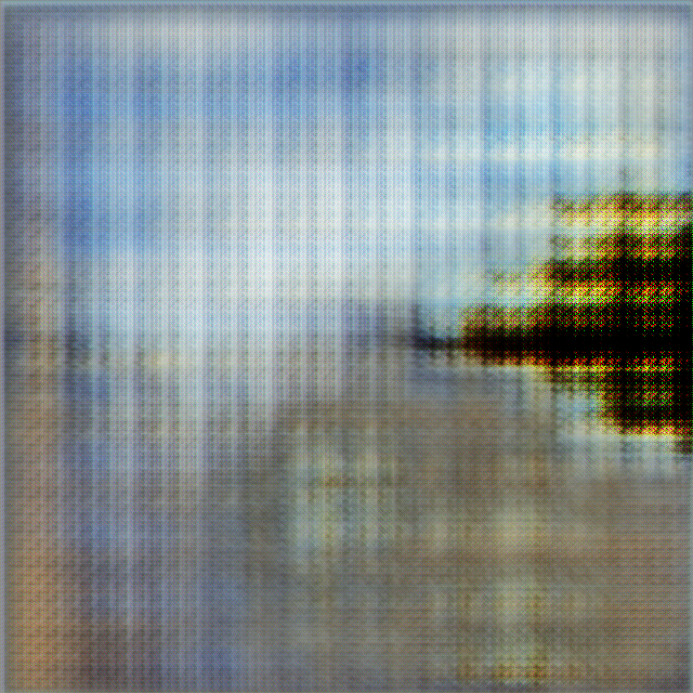
\includegraphics[width=\linewidth]{world_epoch_10_11.png}
            \caption{10 Epochs}
        \end{subfigure} &
        \begin{subfigure}{0.23\textwidth}
            \centering
            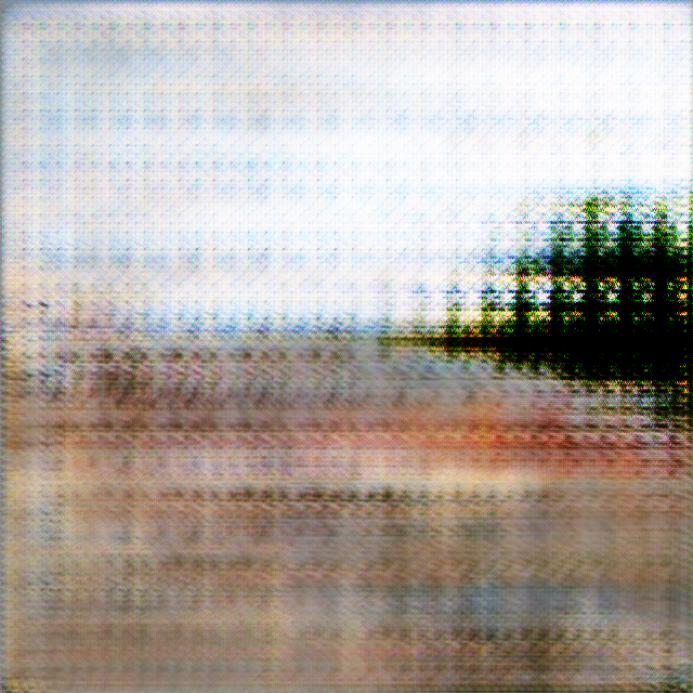
\includegraphics[width=\linewidth]{world_epoch_25_11.png}
            \caption{25 Epochs}
        \end{subfigure} &
        \begin{subfigure}{0.23\textwidth}
            \centering
            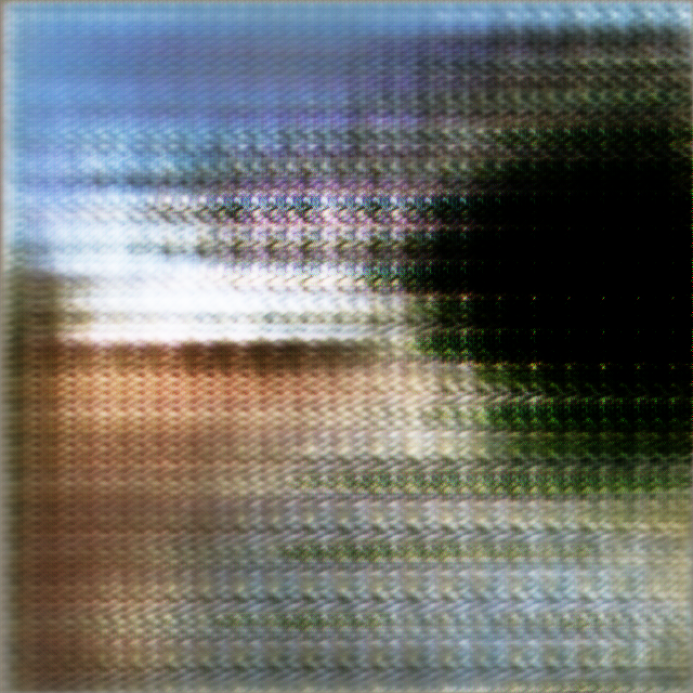
\includegraphics[width=\linewidth]{world_epoch_50_11.png}
            \caption{50 Epochs}
        \end{subfigure} &
        \begin{subfigure}{0.23\textwidth}
            \centering
            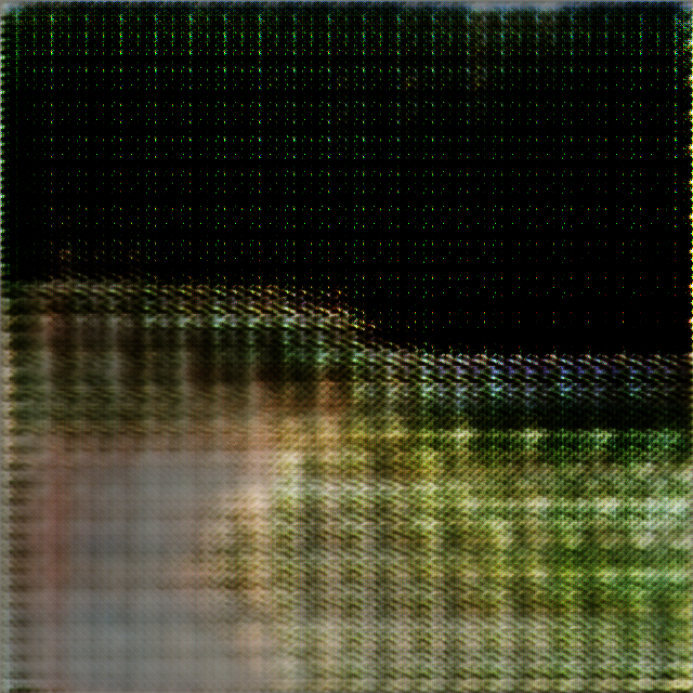
\includegraphics[width=\linewidth]{world_epoch_100_11.png}
            \caption{100 Epochs}
        \end{subfigure} \\
        \begin{subfigure}{0.23\textwidth}
            \centering
            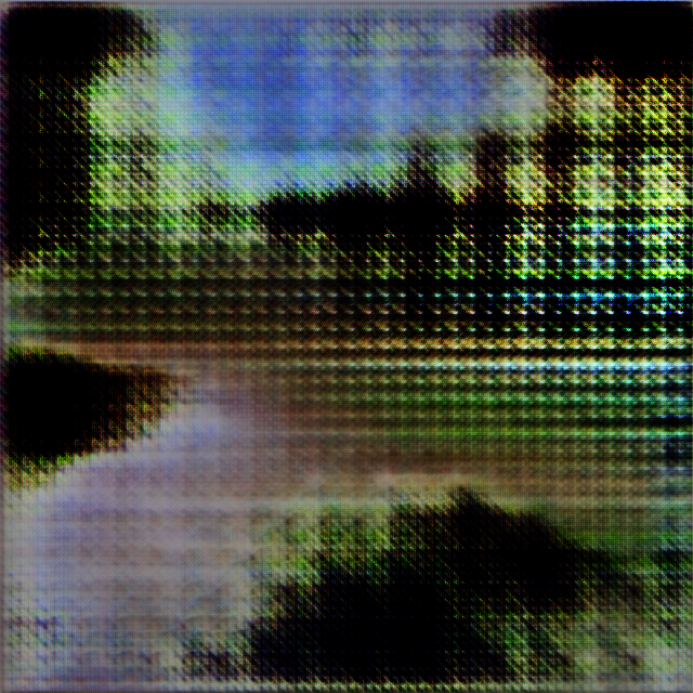
\includegraphics[width=\linewidth]{world_epoch_150_11.png}
            \caption{150 Epochs}
        \end{subfigure} &
        \begin{subfigure}{0.23\textwidth}
            \centering
            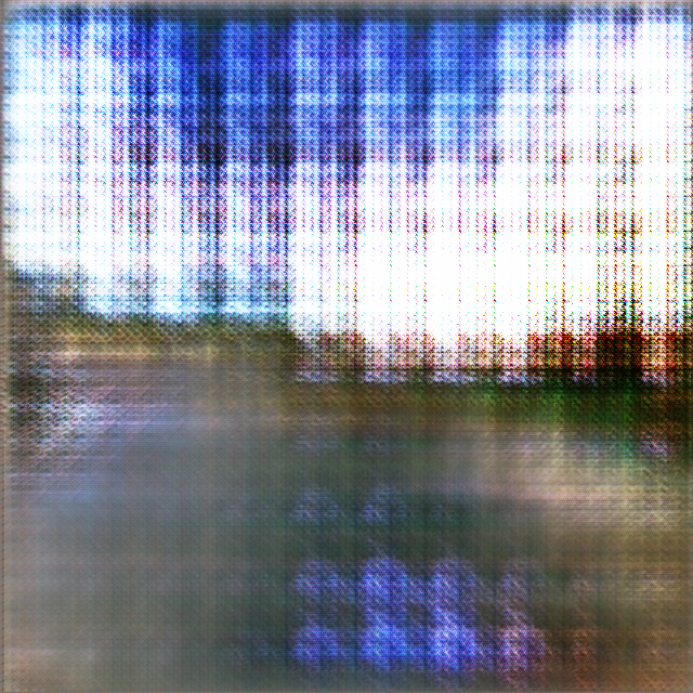
\includegraphics[width=\linewidth]{world_epoch_200_11.png}
            \caption{200 Epochs}
        \end{subfigure} &
        \begin{subfigure}{0.23\textwidth}
            \centering
            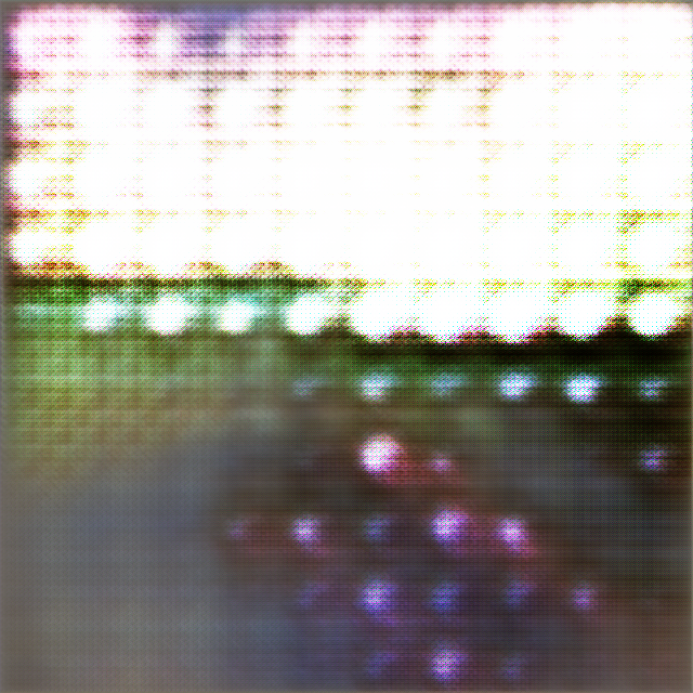
\includegraphics[width=\linewidth]{world_epoch_250_11.png}
            \caption{250 Epochs}
        \end{subfigure} &
        \begin{subfigure}{0.23\textwidth}
            \centering
            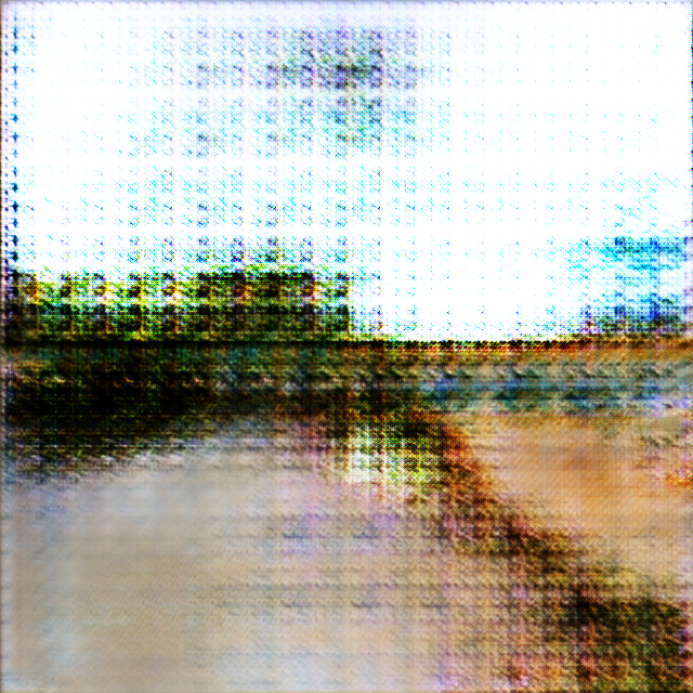
\includegraphics[width=\linewidth]{world_epoch_300_11.png}
            \caption{300 Epochs}
        \end{subfigure} 
    \end{tabular}
    \caption{Training progression over epochs, using the same seed}
    \label{fig:results}
\end{figure}


\end{document}
